\section{Theoretical Analysis}
\label{sec:analysis}

In this section, the circuit shown in Figure 1 is analyzed theoretically with the Mesh Method and with the Nodal Method, in order to complement each other results.

\subsection{Mesh Method}

%The circuit consists of a single V-R-C loop where a current $i(t)$ circulates. The voltage source $v_I(t)$ drives its input, and the output voltage $v_O(t)$ is taken from the capacitor terminals. Applying the Kirchhoff Voltage Law (KVL), a single equation for the single loop in the circuit can be written as

The Mesh Method consists in introducing currents that circulate in the meshes of the circuit, that is, in the loops that do not contain other loops, as shown in Figure~\ref{fig:Circuit_Mesh}, and then evaluate the circuit based on the new currents.

\begin{figure}[h] \centering
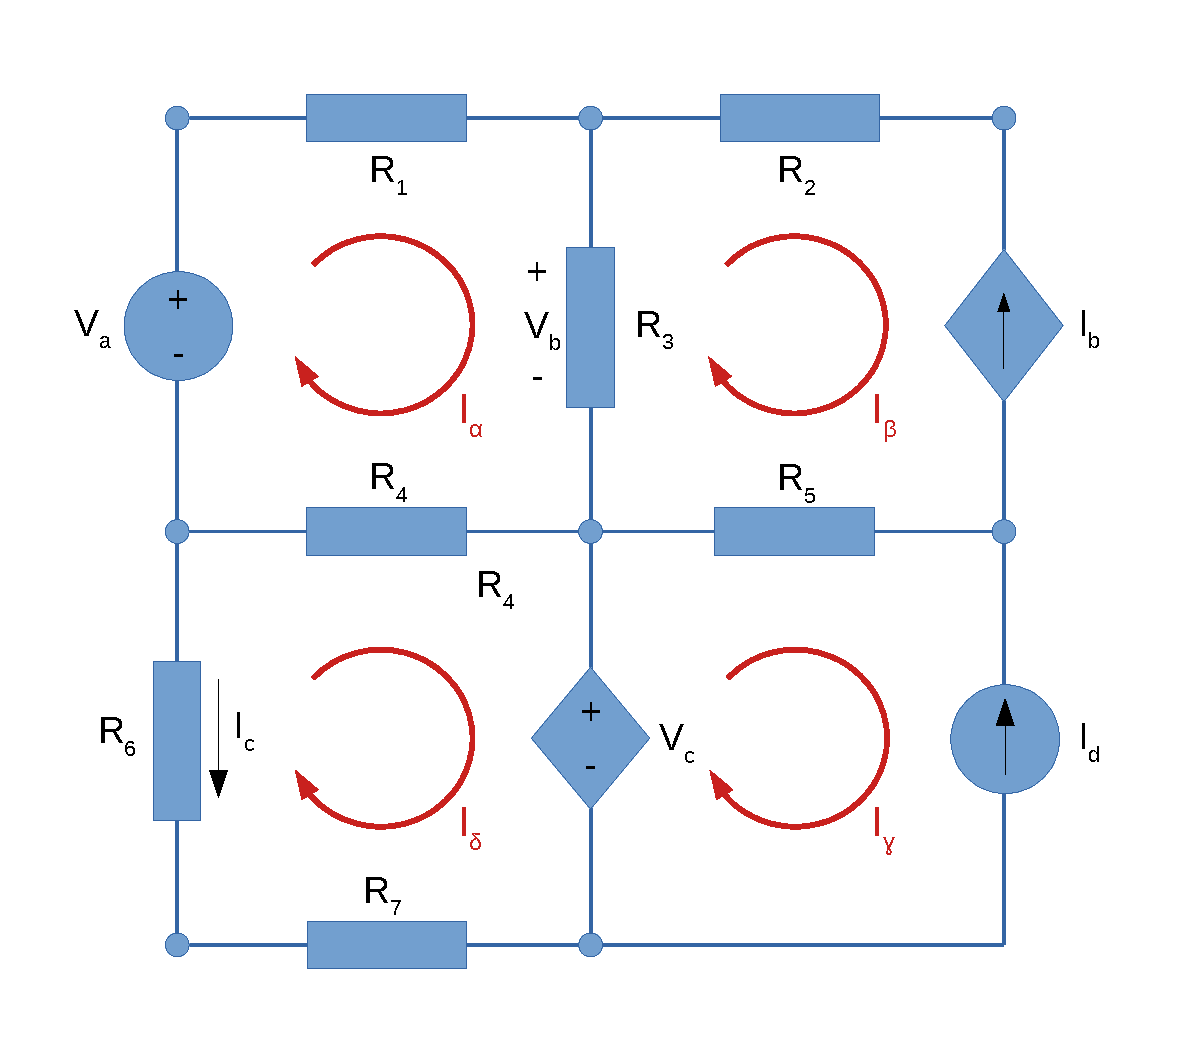
\includegraphics[width=0.5\linewidth]{CircuitMesh.pdf}
\caption{Circuit analysed with mesh currents.}
\label{fig:Circuit_Mesh}
\end{figure}

After identifying the mesh currents, the next step in this method is to use the Kirchhoff Voltage Law~(KVL) in the meshes that do not contain current sources (mesh~$\alpha$~(\ref{eq:MM_Alpha}) and $\delta$~(\ref{eq:MM_Delta})) and to relate the mesh currents to the currents imposed by the sources (mesh~$\beta$~(\ref{eq:MM_Beta}) and $\gamma$~(\ref{eq:MM_Gamma})):

\begin{equation}
  R_1I_{\alpha} + V_b + R_4(I_{\alpha}-I_{\delta}) - V_a = 0
  \label{eq:MM_Alpha}
\end{equation}
\begin{equation}
  R_6I_{\delta} + R_4(I_{\delta}-I_{\alpha}) + V_c + R_7I_{\delta} = 0
  \label{eq:MM_Delta}
\end{equation}

\begin{equation}
  I_{\beta} + I_b = 0;
  \label{eq:MM_Beta}
\end{equation}
\begin{equation}
  I_{\gamma} = - I_d.
  \label{eq:MM_Gamma}
\end{equation}

Since there are 8 variables in the circuit, $I_{\alpha}$, $I_{\beta}$, $I_{\gamma}$, $I_{\delta}$, $V_b$, $V_c$, $I_b$, $I_c$, there must be more four independent equations: two of them are already given,

\begin{equation}
  I_b = K_bV_b;
  \label{eq:Vb_Ib}
\end{equation}
\begin{equation}
  V_c = K_cI_c.
  \label{eq:Vc_Ic}
\end{equation}

The other two are found by examining the circuit and with Ohm's Law:

\begin{equation}
  I_c + I_{\delta} = 0;
  \label{eq:MM_Ic}
\end{equation}
\begin{equation}
  V_b - R_3(I_{\alpha}-I_{\beta}) = 0
  \label{eq:MM_Vb}
\end{equation}

The solution to this linear system of equations is determined by Octave:

\begin{table}[h]
  \centering
  \begin{tabular}{|l|r|}
    \hline    
    {\bf Name} & {\bf Value [A or V]} \\ \hline
    \input{../mat/Malhas_tab}
  \end{tabular}
  \caption{Variables in the Mesh Method. A variable preceded by @ is of type {\em current} and expressed in Ampere; other variables are of type {\em voltage} and expressed in Volt.}
  \label{tab:malhas}
\end{table}

\section{Nodal Method}

In the Nodal Method, the determination of the values of current and voltage is made by, firstly, finding all the knots in the circuit, as made in Figure \ref{fig:Circuit_Nodal}.

\begin{figure}[h] \centering
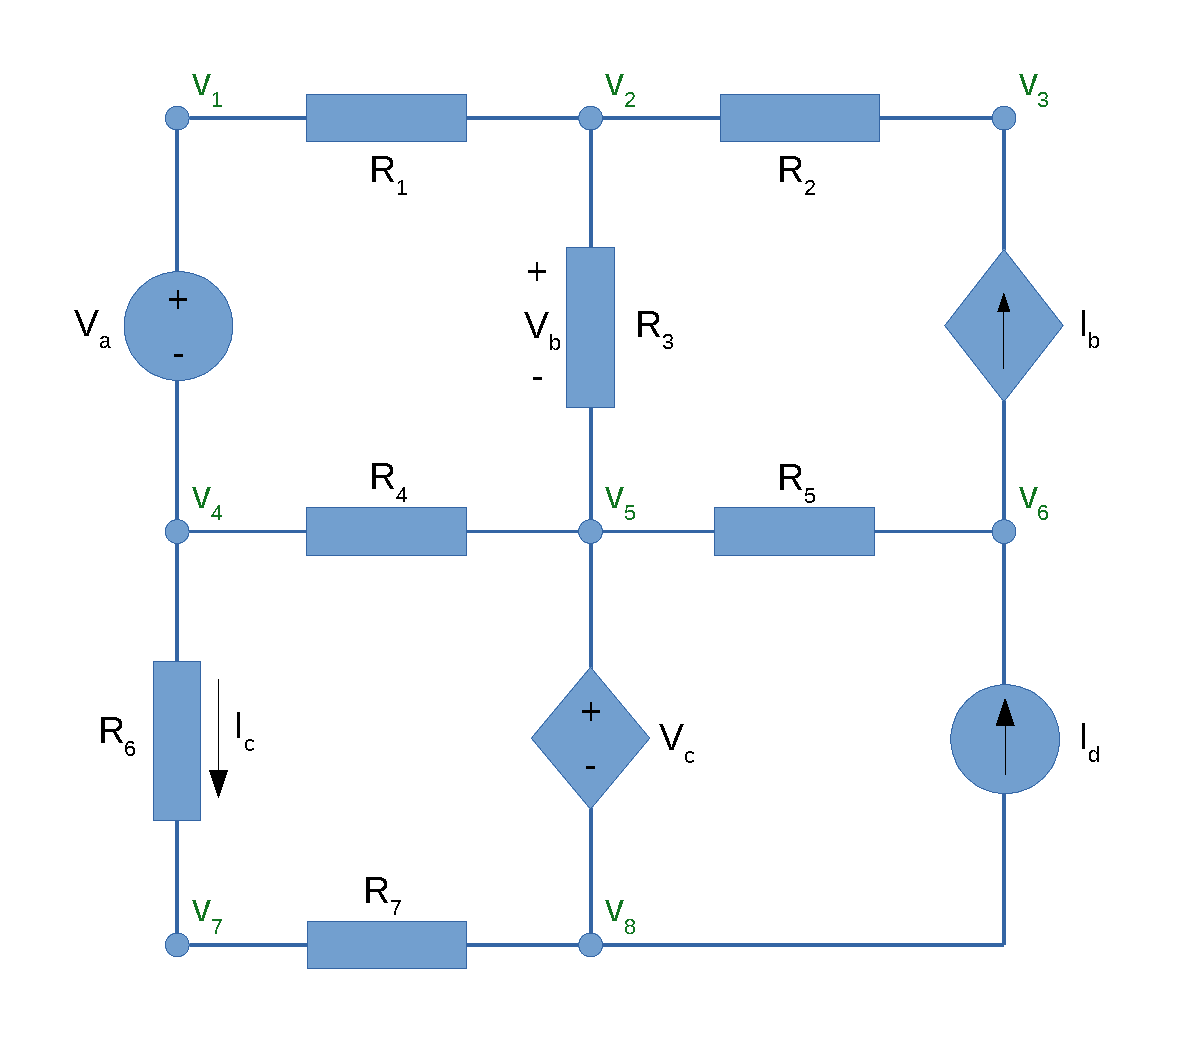
\includegraphics[width=0.5\linewidth]{CircuitNodal.pdf}
\caption{Circuit analysed with nodal voltages.}
\label{fig:Circuit_Nodal}
\end{figure}

Then, it is used the Kirchhoff Current Law~(KCL) in the nodes that are not connected to voltage sources (Equations~\ref{eq:NM_Point2}~to~\ref{eq:NM_Point7}) an relate the knots voltages with the voltage sources that are connected to them (Equations~\ref{eq:NM_Va}~and~\ref{eq:NM_Vc}):

\begin{equation}
  \frac{v_3-v_2}{R_2} - \frac{V_b}{R_3} + \frac{v_1-v_2}{R_1} = 0;
  \label{eq:NM_Point2}
\end{equation}
\begin{equation}
  I_b + \frac{v_2-v_3}{R_2} = 0;	
  \label{eq:NM_Point3}
\end{equation}
\begin{equation}
  \frac{v_5-v_6}{R_5} - I_b = -I_d;
  \label{eq:NM_Point6}
\end{equation}
\begin{equation}
  I_c + \frac{v_8-v_7}{R_7} = 0;
  \label{eq:NM_Point7}
\end{equation}

\begin{equation}
  v_1 - v_4 = V_a;
  \label{eq:NM_Va}
\end{equation}
\begin{equation}
  v_5 - v_8 - V_c = 0.
  \label{eq:NM_Vc}
\end{equation}

Since there are 8+4 variables ($v_1$~to~$v_8$, $V_b$, $V_c$, $I_b$, $I_c$), the system is defined by twelve independent equations. Two are provided in the circuit and are the same as in the Mesh Method, (\ref{eq:Vb_Ib})~and~(\ref{eq:Vc_Ic}).
By observing the circuit,
\begin{equation}
  v_5 - v_8 - V_b = 0.
  \label{eq:NM_Vb}
\end{equation}

Using Ohm’s Law, we find the relation:
\begin{equation}
  I_c - \frac{v_4-v_7}{R_6} = 0.
  \label{eq:NM_OhmIc}
\end{equation}

Because there needs to be a knot with a defined voltage, we chose $v_4$ to be connected to the ground:
\begin{equation}
  v_4 = 0.
  \label{eq:NM_v4=0}
\end{equation}

For the last equation, the continuity of current in the circuit can be used to create a “super-knot”, bypassing the voltage sources.

\begin{equation}
  \frac{v_5-v_4}{R_4} + \frac{v_2-v_1}{R_1} - I_c = 0;
  \label{eq:NM_SPVa}
\end{equation}
\begin{equation}
  \frac{v_7-v_8}{R_7} - Id + \frac{v_6-v_5}{R_5} + \frac{Vb}{R3} + \frac{v_4-v_5}{R_4} = 0.
  \label{eq:NM_SPVc}
\end{equation}

Given that there only one equation is needed, we chose to use the more simple~(\ref{eq:NM_SPVa}.
The solution to this linear system of equations is determined by Octave:

\begin{table}[h]
  \centering
  \begin{tabular}{|l|r|}
    \hline    
    {\bf Name} & {\bf Value [A or V]} \\ \hline
    \input{../mat/Nos_tab}
  \end{tabular}
  \caption{Variables in the Nodal Method. A variable preceded by @ is of type {\em current} and expressed in Ampere; other variables are of type {\em voltage} and expressed in Volt.}
  \label{tab:nos}
\end{table}

